\documentclass[11pt]{article}
\usepackage[english]{babel}  % Croatian typographical rules and hyphenation patterns
\usepackage{ae,aecompl}     	% Type 1 fonts, similar to Computer Modern

\usepackage{microtype}				% Improves spacing

\usepackage{booktabs}					% Nice looking tables
\usepackage{enumerate}				% Additional options for listing of items in enumerate environment
\usepackage{algorithm2e}			% Writing pseudo-code
\usepackage{todonotes}				% Adding todo items
\usepackage{dirtree}					% Simple display of directory tree
\usepackage{hyperref}

\usepackage{graphicx}
\usepackage{subfig}
\usepackage{caption}
\usepackage{listings}

\hypersetup{
    colorlinks=true,
    linkcolor=blue,
    filecolor=magenta,
    urlcolor=cyan,
}
\urlstyle{same}
\usepackage{graphics}

\graphicspath{ {./images/} }

\title{
	\Large Josip Juraj Strossmayer University of Osijek \\
	Faculty of Electrical Engineering, Computer Science and Information
	 Technologies\\
	\vspace{4cm}
	\Large Course: Linux in Embedded Systems \\
	\vspace{4cm}
	\Large \textbf{Laboratory exercise 2: Getting familiar with Raspberry Pi
		3.\\
		Building Linux for Raspberry Pi 3}
	}
\date{}
\begin{document}
\maketitle
\thispagestyle{empty}
\newpage

\section{Introduction}
The Raspberry Pi computer was launched in early 2012 and launched a revolution
 in the field of computer related education and hobbies. This computer has
 become extremely popular because of its price (around \$35) and small
 dimensions (8.6cm x 5.4cm x 1.7cm). Although the Raspberry Pi is a
 general-purpose computer, it has the ability to connect different equipment
 (e.g. different sensors and actuators) so it is used in many hobby projects in
 different embedded computer systems and IoT (Internet of Things) areas, and
 increasingly in various commercial projects. The main part of this computer
 represents SoC (System On a Chip) with a different periphery like
 RAM, HDMI output, Ethernet port, etc. Also on the board there are General
 Purpose Input Output (GPIO) pins that enable connecting different equipment.

\section{Raspberry Pi Models}
To date, several generations of Raspberry Pi computers have been released.
 All in common with Broadcom SoC consisting integrated ARM processor (CPU)
 and a built-in GPU. The processor clock speed is moving from 700 MHz to 1.4 GHz
 for Pi 3B+ or 1.5 GHz for Pi 4. The amount of memory (RAM) ranges from 256 MB
 to 1 GB or even 4 GB code on strongest model of the latest Pi 4. Secure Digital
 (SD) cards are used for storage of the operating system and programs.
 There are up to four USB ports on the board. HDMI is used for video output.
 Using GPIO pins standard protocols such as I\textsuperscript{2}C are supported.
 All B models have Ethernet connection, while the Pi 3 and Pi Zero W have Wi-Fi
 802.11n and Bluetooth.
\newline
\newline
Smaller-sized Raspberry Pi Zero with reduced set of input-output units and
 general purpose input and output units (GPIO) was released to market in 2015
 with a price tag of \$5. In 2017, the Raspberry Pi Zero W with added Wi-Fi and
 Bluetooth capabilities was released.
The Raspberry Pi 3 Model B was released in 2016 with 1.2 GHz 64-bit quad-core
 processor and built-in 802.11n Wi-Fi and Bluetooth capabilities. In 2018, the
 Raspberry Pi 3 Model B+ with 1.4 GHz processor and gigabit Ethernet
network (by actual tests it reaches a speed of 300 Mbit/s because it shares a
USB 2.0 bus) was released.
 It comes with dual-band 802.11ac 2.4/5 Ghz Wi-Fi wireless networking.
\begin{figure}[h!]
\centering
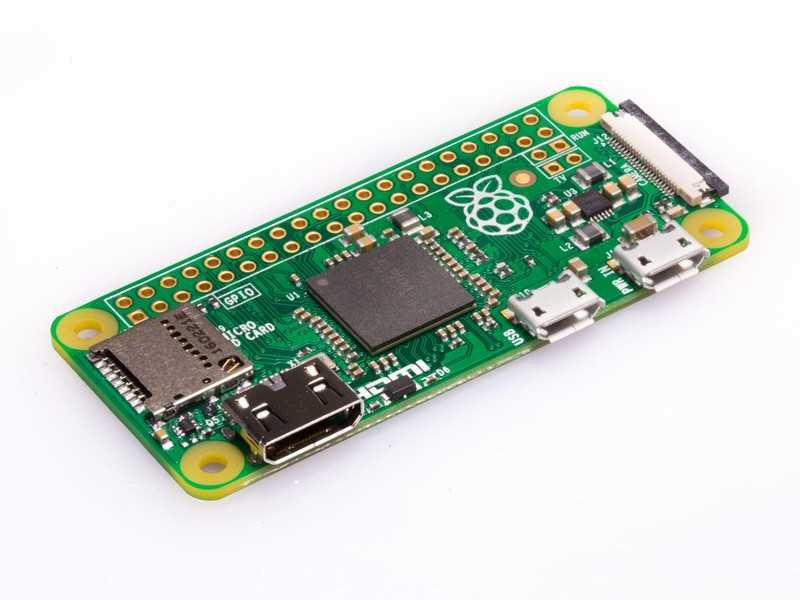
\includegraphics[width=0.8\textwidth]{rpi-zero.jpg}
\captionsetup{justification=centering}
\caption{Raspberry Pi Zero}
\end{figure}
The latest Raspberry Pi Model 4 B was released in 2019. It has 1.5 GHz
 quad-core ARM Cortex-A72 processor, 802.11ac supported Wi-Fi,
 Bluetooth 5 support, fully supported Gigabit Ethernet, two USB 2.0 ports, two
 USB 3.0 ports and a support for 4K video resolution.
\newline
\newline
On laboratory exercises \textbf{Raspberry Pi 3 B} will be used.
\newline
\newline
Technical specifications of Raspberry Pi 3 B: \\
\textbf{SoC}: Broadcom BCM2837 \\
\textbf{CPU}: quad-core ARM Cortex-A53, 1.2GHz \\
\textbf{GPU}: Broadcom VideoCore IV \\
\textbf{RAM}: 1GB LPDDR2 (900 MHz) \\
\textbf{Network}: 10/100 Ethernet, 2.4GHz 802.11n wireless \\
\textbf{Bluetooth}: Bluetooth 4.1 Classic, Bluetooth Low Energy \\
\textbf{Storage}: MicroSD \\
\textbf{GPIO}: 40-pin header, populated \\
\textbf{I/O}: $4\times USB 2.0$, HDMI, 3.5mm analogni priključak,
 Ethernet, \textit{Camera Serial Interface} (CSI), \textit{Display Serial
 Interface} (DSI)

 \begin{figure}[h!]
\centering
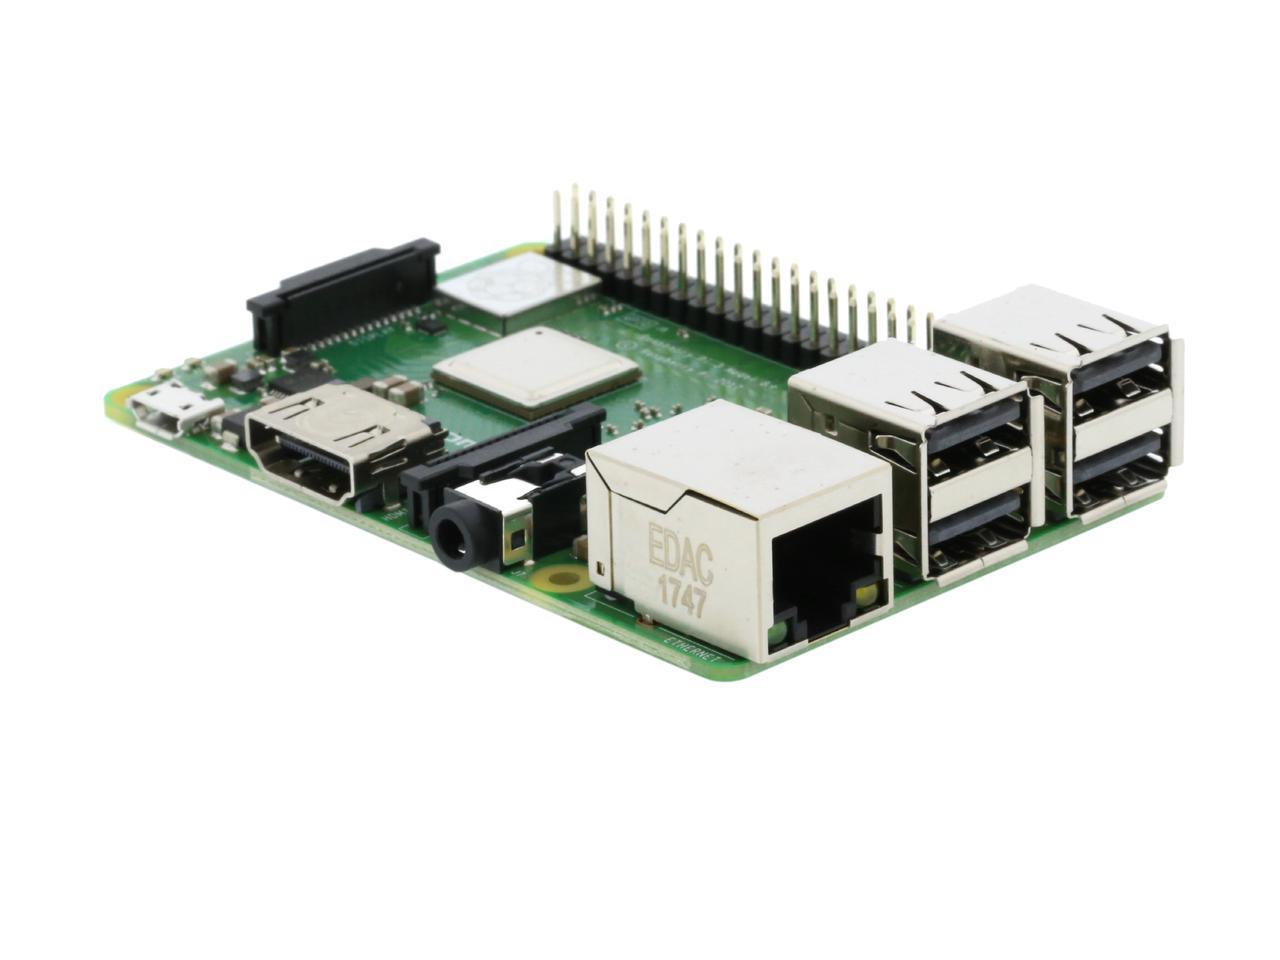
\includegraphics[width=0.8\textwidth]{rpi-3-b-plus.jpg}
\captionsetup{justification=centering}
\caption{Raspberry Pi 3 B+}
\end{figure}
\begin{figure}[h!]
\centering
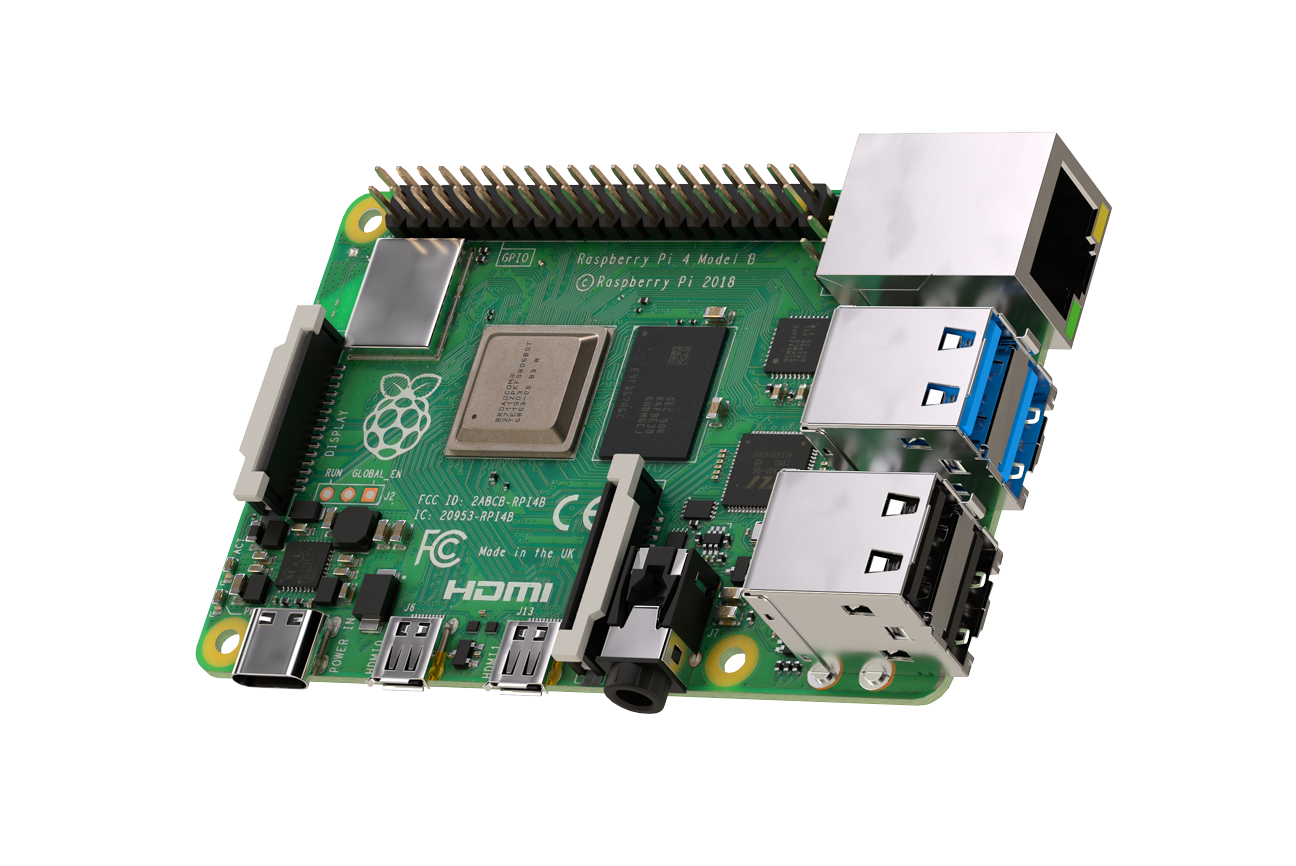
\includegraphics[width=0.8\textwidth]{rpi-4.png}
\captionsetup{justification=centering}
\caption{Raspberry Pi 4 B}
\end{figure}

\begin{figure}
\centering
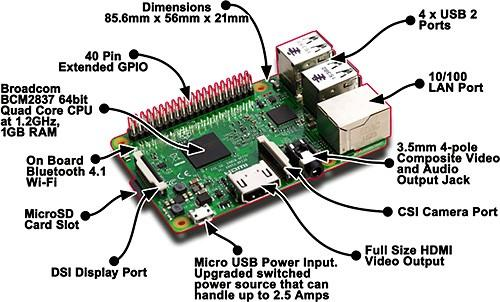
\includegraphics[width=0.8\textwidth]{rpi-3-details.jpg}
\captionsetup{justification=centering}
\caption{Raspberry Pi 3 details}
\end{figure}
\begin{figure}[h!]
	\centering
	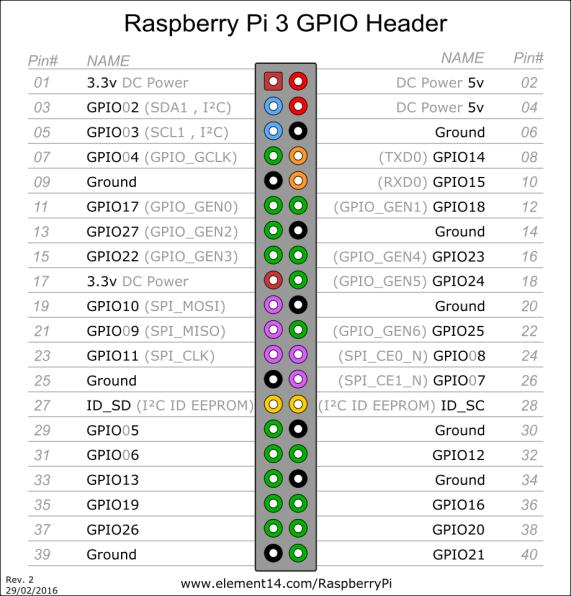
\includegraphics[width=0.8\textwidth]{rpi-3-pins.jpg}
	\captionsetup{justification=centering}
	\caption{Raspberry Pi 3 GPIO}
	\label{fig:rpi-gpio}
\end{figure}

\clearpage
\section{Additional equipment}
Apart from the Raspberry Pi itself, various accessories are required
depending on the application:
\begin{enumerate}
	\item power supply 5V 2A, USB micro connector
	\item micro SD memory card, capacity min. 4GB Class A
	\item USB converter to serial cable communication (UART)
	\item USB converter to Ethernet and Ethernet cable
	\item additional driver development devices.
\end{enumerate}

\begin{figure}
    \centering
    \subfloat[Power supply]{{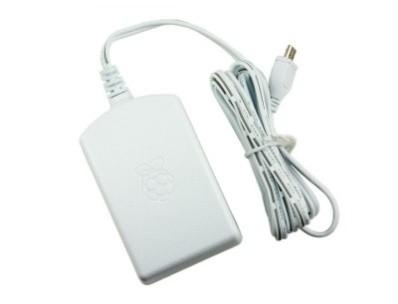
\includegraphics[width=4cm]{rpi-charger.jpg}}}%
    \subfloat[SD card]{{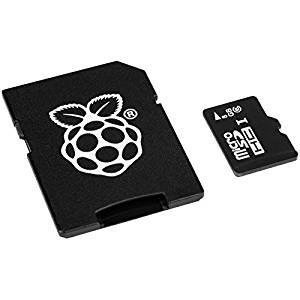
\includegraphics[width=4cm]{rpi-sdcard.jpg}}}%
    \subfloat[USB UART]{{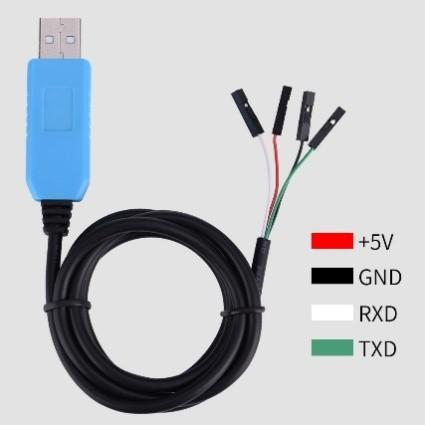
\includegraphics[width=4cm]{rpi-uart.jpg}}}%
    \qquad
    \subfloat[USB Ethernet]{{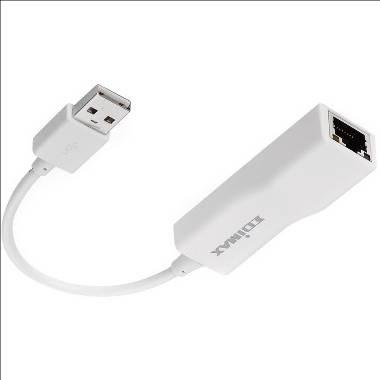
\includegraphics[width=4cm]{rpi-ethernet.jpg}}}%
    \subfloat[Nunchuk]{{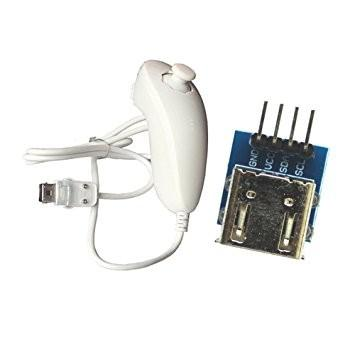
\includegraphics[width=4cm]{rpi-nunchuk.jpg}}}%
    \subfloat[Case]{{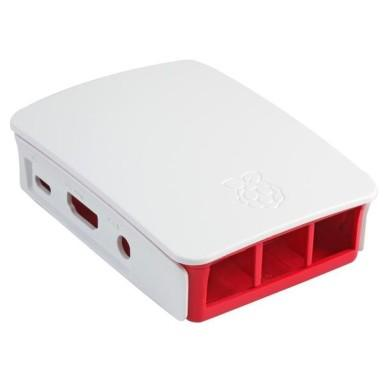
\includegraphics[width=4cm]{rpi-case.jpg}}}%
    \caption{Raspberry Pi accessories}%
    \label{fig:equipment1}%
\end{figure}

\section{Initial setup}
If you don't have your \texttt{embedded\_linux} repository on your development
 computer, first clone it with the appropriate command from your Gitlab account
 into your \textit{home} directory. Position yourself in the\\
 \texttt{/home/rtrk/embedded\_linux} directory. Then pull the possible changes
 from the source repository using the command:
\begin{lstlisting}[language=bash]
git remote add upstream
	https://gitlab.com/rgrbic/embedded_linux
git fetch upstream
git merge upstream/master
\end{lstlisting}
Install additional tools using command:
\begin{lstlisting}[language=bash]
sudo apt-get install gcc-arm-linux-gnueabihf
\end{lstlisting}

\section{Buildroot}
The Build system is a toolkit that allows you to automate the Linux build
 process for embedded computing systems. More specifically, build systems allow
 you to build toolchain tools, bootloaders, kernels, and root filesystems based
 on source code. Some of the better known build systems are Buidroot, Yocto,
 PTXdist and OpenEmbedded.
\newline
\newline
For the purpose of building Linux for Raspberry Pi computer theBuildroot tool
 will be used. Open the terminal and download Buildroot using the command:
\begin{lstlisting}[language=bash]
git clone https://github.com/buildroot/buildroot
\end{lstlisting}
Once the cloning process on your development computer is complete, enter
cloned directory:
\begin{lstlisting}[language=bash]
cd buildroot
\end{lstlisting}
You will notice that this directory has several subdirectories (use the
 \texttt{ls} command) of which the most important are (details can be viewed at
 \url{https://buildroot.org/downloads/manual/manual.html}):
\newline
\newline
\texttt{dl/}: contains archives of upstream projects that Buildroot has built
\newline
\newline
\texttt{output/}: output files of compiled code
\newline
\newline
\texttt{host/}: these are various tools required by Buildroot that run on the
 host computer, including toolchain executables
 (\texttt{output/host/usr/bin})
\newline
\newline
\texttt{images/}: this is the most important directory because it contains the
 build results (depending on what is selected in the Bootloader configuration:
 bootloader, kernel and one or more root filesystems)
\newline
\newline
\texttt{staging/}: this is a symbolic link to the toolchain sysroot
\newline
\newline
\texttt{target/}: this is almost a complete root file system (however, it is
 not intended to be used as a root file system on a target computer)
\newline
\newline
\texttt{configs/}: here are predefined configurations for different panels
 (e.g. raspberrypi3 defconfig)
\newline
\newline
\texttt{boards/}: here are various scripts that define how to generate system
 images (sdcard.img), post build procedures, etc.
\newline
\newline
Although it can be used to build Linux using Buildroot \\
 \texttt{raspberrypi3\_defconfig} which is further modified according to user
 preferences with the \texttt{make menuconfig|nconfig|xconfig}, existing
 configuration will be used in this exercise. Copy
 \texttt{raspberrypi3\_ferit\_defconfig} file from directory
 \texttt{/home/rtrk/embedded\_linux/LV2/resources} into directory
 \texttt{/home/rtrk/buildroot/configs}. Furthermore, copy the files
 \texttt{post-build.sh} and \texttt{genimage-raspberrypi3.cfg} to the
 directory \texttt{/home/rtrk/buildroot/board/raspberrypi}.\\
\newline
Load the given configuration and see what is included in it by running the
 following commands in the \texttt{/home/rtrk/buildroot} directory:
\begin{lstlisting}[language=bash]
make raspberrypi3_ferit_defconfig
make menuconfig
\end{lstlisting}
Start the build using command:
\begin{lstlisting}[language=bash]
make
\end{lstlisting}
Because Buildroot needs to fetch all the source code of different components
 (toolchain, bootloader, kernel, etc.), this command may take some time
 depending on the speed of the internet connection and the speed of the
 development computer. During this time, get to know the Raspberry Pi and
 how to build individual Linux components.
\newline
\newline
Locate the 40 pin header on the Raspberry Pi board (\ref{fig:rpi-gpio}) and
 identify the serial communication (RXD, TXD) pins. Connect the USB converter
 to the serial connection by connecting:\\
\newline
USB-serial GND $\leftrightarrow$ GND Raspberry Pi \\
USB-serial TXD $\leftrightarrow$ RX0 Raspberry Pi \\
USB-serial RXD $\leftrightarrow$ TX0 Raspberry Pi \\
\textbf{\textcolor{red}{(Do not connect +5V of the USB-serial to Raspberry
 Pi!)}} \\
\newline
Open a new terminal. Install the picocom serial communication tool
using the command:
\begin{lstlisting}[language=bash]
sudo apt-get install picocom
\end{lstlisting}
Test the serial connection by connecting the converter to the development
 computer. At the terminal, execute the command:
\begin{lstlisting}[language=bash]
picocom -b 115200 /dev/ttyUSB0
\end{lstlisting}
If the converter is correctly recognized, “Terminal ready” will be displayed.
 Disconnect the USB converter, the serial connection should be disconnected at
 the terminal. If you want to leave picocom without disconnecting the converter
 from USB, press Ctrl+a followed by Ctrl+x.
\newline
\newline
Once the Linux build is completed using the Buildroot tool, the following files
 will be located in the \texttt{/home/rtrk/buildroot/output/images} directory:
\newline
\dirtree{%
	.1 images.
	.2 bcm2710-rpi-3-b.dtb.
	.2 boot.vfat.
	.2 rootfs.ext2.
	.2 rootfs.ext4.
	.2 rpi-firmware.
	.3 bootcode.bin.
	.3 cmdline.txt.
	.3 config.txt.
	.3 fixup.dat.
	.3 start.elf.
	.3 overlays.
	.2 sdcard.img.
	.2 u-boot.bin.
	.2 zImage.
}%\\
The sdcard.img file contains all of the above Linux components and needs to be
 written to a micro SD card. Insert the micro SD card into the memory card
 reader and connect it to the development computer (usually \texttt{/dev/sdX}
 where \texttt{X} is a, b, c, etc.). Copy the file to the micro SD card with
 the following commands:
\begin{lstlisting}[language=bash]
sudo dd status=progress if=sdcard.img of=/dev/sdx
sudo sync
\end{lstlisting}
If you have trouble writing files using the previous commands, then it is
 recommended that you install GParted, which is a graphical disk manipulation
 tool:
\begin{lstlisting}[language=bash]
sudo apt-get install gparted
\end{lstlisting}
After installation, run the Gparted tool from the Ubuntu graphics environment
 and wipe all the partitions on your micro SD card (
 \textbf{\textcolor{red}{Caution! Be sure to delete the partitions on the micro
 SD card other than your computer's storage media such as your hard disk!}}).
\newline
\newline
When the file copy is successfully completed, your micro SD card will have
 two partitions, with the first partition containing the files required to load
 the OS (firmware, bootloader, and the kernel itself), while the second
 partition will have the root file system. Securely unplug the memory card
 reader from your PC, remove the micro SD card, and insert it into the
 Raspberry Pi. Connect the PC and Raspberry Pi via USB to a serial connection,
 then connect the PC and Raspberry Pi via USB to Ethernet converter.
Open a serial connection in a new terminal on your PC using the command:
\begin{lstlisting}[language=bash]
picocom -b 115200 /dev/ttyUSB0
\end{lstlisting}
Connect the power to the Raspberry Pi. After a while, the status messages of
 the U-boot bootloader should appear in the terminal where the serial
 connection is open and the command line beginning with \texttt{U-boot>}. Press
 Enter to stop the autoboot.

\section{U-boot configuration}
Typing the \texttt{help} command into the U-boot command prompt will display a
 list of available commands. Eg. the list of all environment variables is
 obtained by the command:
\begin{lstlisting}[language=bash]
printenv
\end{lstlisting}
Changing the environment variable is done using the \texttt{setenv} or
 \texttt{editenv} command. For example:
\begin{lstlisting}[language=bash]
setenv boodelay 4
\end{lstlisting}
Save the environment after changing the variables to have the values set when
 restarting the U-boot. Save the environment to a micro SD card with the
 command:
\begin{lstlisting}[language=bash]
saveenv
\end{lstlisting}
In order to run Linux, you need to define a bootargs environment variable and
 define bootcmd that will load zImage and the corresponding device tree blob to
 the appropriate addresses:
\begin{lstlisting}[language=bash]
setenv bootargs "8250.nr_uarts=1 root=/dev/mmcblk0p2
console=ttyS0,115200 rootfstype=ext4 elevator=deadline
fsck.repair=yes rootwait"

setenv bootcmd "fatload mmc 0:1 0x01000000 zImage;
fatload mmc 0:1 0x2000000 bcm2710-rpi-3-b.dtb;
bootz 0x01000000 - 0x2000000"
\end{lstlisting}
Save the environment with the saveenv command and then run Linux with the
 command:
\begin{lstlisting}[language=bash]
run bootcmd
\end{lstlisting}
At the terminal you will get a print about booting the Linux kernel and setting
 up the root file system. Upon completion of the boot, you will receive a line
 to log on to the system named buildroot. Use a root username, without a
 password.
\begin{lstlisting}[language=bash]
Welcome to Buildroot

buildroot login: root

buildroot:~#
\end{lstlisting}
The file system contains basic commands within BusyBox. Try to list the
 contents of the directory and find BusyBox. When you're done, type
 \texttt{poweroff} so you can safely unplug the board. Turn on the power on the
 board again, and when the countdown starts in the U-boot, stop it by pressing
 any key (in case of expiration of time the \texttt{bootcmd} will be
 executed).

\section{Setting up and using TFTP protocol with Raspberry Pi}
With Linux development, kernel image changes are common, which requires copying
 the image to a micro SD card. In order to avoid frequent transfer of the micro
 SD card from the Raspberry Pi to the memory card reader and vice versa, it is
 possible to configure the U-boot and the development computer so that the
 files are transferred by TFTP (Trivial File Transfer Protocol) protocol.
 First, install the TFTP server on the development computer:
\begin{lstlisting}[language=bash]
sudo apt-get install tftpd-hpa
\end{lstlisting}
Using a network cable, connect the Raspberry Pi and the development PC using a
 USB to Ethernet converter. Connect the Raspberry Pi to the development PC
 using a USB converter to a serial connection. Open the terminal and start the
 picocom serial terminal with the appropriate command. Connect the power to the
 Raspberry Pi. Press a button on your computer to stop automatic booting on the
 Raspberry Pi. A new network will appear on the development computer
 connection. Set up this network connection as shown in
 \ref{fig:ubuntu-ethernet}. In the IPv4 Settings tab, select Manual as the
 method to enable a static IP address, eg 192.170.0.1 (of course, make sure
 that this address belongs to a different network segment than the main network
 to which it is already a development computer connected). For Netmask, set 24
 and leave the Gateway field blank. The U-Boot command line requires setting
 environment variables that match the IP address of the client (Raspberry Pi)
 and server (development computer), for example:
\begin{lstlisting}[language=bash]
setenv ipaddr 192.170.0.100
setenv serverip 192.170.0.1
\end{lstlisting}
\begin{figure}[h!]
\centering
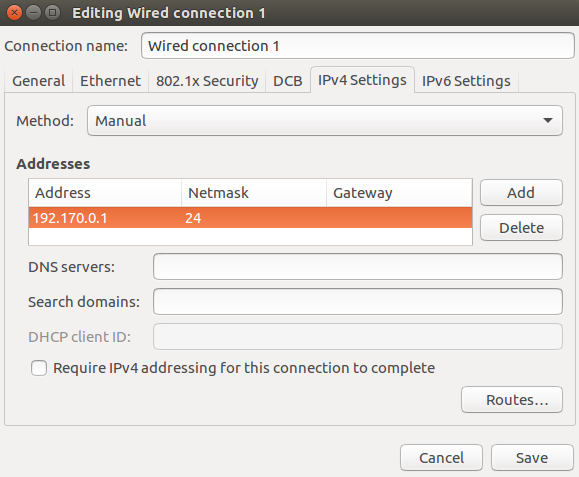
\includegraphics[width=0.8\textwidth]{ubuntu-ethernet.png}
\captionsetup{justification=centering}
\caption{USB Ethernet network connection settings}
\label{fig:ubuntu-ethernet}
\end{figure}
Save these changes to the micro SD card with the command:
\begin{lstlisting}[language=bash]
saveenv
\end{lstlisting}
Check for changes using the command:
\begin{lstlisting}[language=bash]
printenv
\end{lstlisting}
Test whether the TFTP connection is working properly. Create a small text file
 in \texttt{/var/lib/tftpboot} called \texttt{file\_example.txt}. Use the
 U-boot command prompt to execute the following command:
\begin{lstlisting}[language=bash]
tftp 0x01000000 file_example.txt
\end{lstlisting}
This command should move the \texttt{file\_example.txt} file from the
 development computer to the Raspberry Pi board to the memory location
 0x01000000 (this location belongs to the DRAM on the board). Verify this entry
 by reading content from this address:
\begin{lstlisting}[language=bash]
md 0x01000000
\end{lstlisting}
You can also check the connection using the \texttt{ping} command. On the
 Raspberry Pi (in the U-boot), execute the command:
\begin{lstlisting}[language=bash]
ping 127.0.0.1
\end{lstlisting}
On the development computer, execute the command:
\begin{lstlisting}[language=bash]
ping 127.0.0.1
\end{lstlisting}
Since the Raspberry Pi network is only occasionally active, try the above
 commands at about the same time. In case of problems with
 \texttt{file\_example.txt} file transfer and communication:\\
\newline
1) Check the IP address of the server and client that are configured in the
 U-boot.
\newline
2) Use the \texttt{ls /var/lib/tftpboot} command to check for a file you want
 to transfer.
\newline
3) Restart the tftpd-hpa service with the command:
 \texttt{sudo service tftpd-hpa restart}.

\section{NFS Server and File System setup}
Untar the built-in root filesystem into the appropriate directory (assuming you
 are in your home directory):
\begin{lstlisting}[language=bash]
sudo tar xvjf buildroot/output/images/rootfs.tar.bz2 -C
embedded_linux/LV2/solutions/nfsroot
\end{lstlisting}
Change the rights in the directory:
\begin{lstlisting}[language=bash]
sudo chown -R rtrk embedded_linux/LV2/solutions/nfsroot/root
\end{lstlisting}
Install the NFS Server using command:
\begin{lstlisting}[language=bash]
sudo apt-get install nfs-kernel-server
\end{lstlisting}
Modify the \texttt{/etc/exports} file as a root user by adding the following
 line:
\begin{lstlisting}[language=bash]
/home/rtrk/embedded_linux/LV2/solutions/nfsroot
<IP_address_rpi>(rw,no_root_squash,no_subtree_check)
\end{lstlisting}
wherein the \texttt{<IP\_adresa\_rpi>} is the Raspberry Pi IP address. Again
run the NFS server using the command:
\begin{lstlisting}[language=bash]
sudo /etc/init.d/nfs-kernel-server restart
\end{lstlisting}
\section{Boot and load the root file systems via NFS}
Run the board to the U-boot. Before launching the kernel, it is necessary to
 define which console to use and which root filesystem to boot through NFS. Set
 the U-boot bootagrs environment variable as follows:
\begin{lstlisting}[language=bash]
setenv bootargs "root=/dev/nfs rw ip=<IP_address_rpi> 8250.nr_uarts=1
console=ttyS0,115200
nfsroot=<IP_address_pc>:/home/rtrk/embedded_linux/LV2/solutions/nfsroot"

saveenv
\end{lstlisting}
If you want to change the settings later, you can change the variables with:
\begin{lstlisting}[language=bash]
editenv bootargs
\end{lstlisting}
Now transfer the kernel image through TFTP:
\begin{lstlisting}[language=bash]
tftp 0x01000000 zImage
\end{lstlisting}
Device tree blob needs to be transferred also:
\begin{lstlisting}[language=bash]
tftp 0x2000000 bcm2710-rpi-3-b.dtb
\end{lstlisting}
You can now run the kernel:
\begin{lstlisting}[language=bash]
bootz 0x01000000 - 0x2000000
\end{lstlisting}
If everything is OK, an login prompt will appear (user: root, no password).
If the kernel fails to boot the network file system, terminal error messages
 will appear. Also see the NFS server messages in \texttt{/var/log/syslog} on a
 development computer:
\begin{lstlisting}[language=bash]
cat /var/log/syslog
\end{lstlisting}
You can check that the network file system works by adding a text file to the
 root directory of the network file system and typing arbitrary text into it:
\begin{lstlisting}[language=bash]
sudo nano /home/rtrk/embedded_linux/LV2/solutions/nfsroot/root/test.txt
\end{lstlisting}
On the Raspberry Pi, the same file should be in the \texttt{/root} directory,
 for example, execute the command:
\begin{lstlisting}[language=bash]
cat /root/test.txt
\end{lstlisting}

\section{Boot automatically}
To avoid typing the same commands every time the board is turned on, you can
 use the U-boot bootcmd variable:
\begin{lstlisting}[language=bash,escapechar=\&]
setenv bootcmd "tftp 0x01000000 zImage;&\newline&tftp 0x2000000 bcm2710-rpi-3-b.dtb;bootz 0x01000000 - 0x2000000"

saveenv
\end{lstlisting}
Feel free to change this as needed. Eg. if you want to restore startup from a
 micro SD card:
\begin{lstlisting}[language=bash]
setenv bootargs "8250.nr_uarts=1 root=/dev/mmcblk0p2 console=ttyS0,115200
rootfstype=ext4 elevator=deadline fsck.repair=yes rootwait"

setenv bootcmd "fatload mmc 0:1 0x01000000 zImage; fatload mmc 0:1
0x2000000 bcm2710-rpi-3-b.dtb; bootz 0x01000000 - 0x2000000"

saveenv
\end{lstlisting}

\end{document}
